\thispagestyle{empty}
\begin{center}
    \Large
    \textbf{Simulation of complex actuators}
    
    \vspace{0.4cm}
    \large
    Hubert Woszczyk, under the supervision of Prof. Bernard Boigelot
    
    \normalsize
    Academic year 2015-2016\\
    Faculty of Applied Sciences\\
    Electrical Engineering
    
    \vspace{0.9cm}
    \textbf{Abstract}
\end{center}
The word \emph{robot} has been crafted by Czech writer Karel Čapek in the beginning of the 20th century and is derived from the slavic world \emph{robota} which means \emph{work}, as in \emph{there is work to be done}. Much has changed since those days, and this master's thesis is about robots who prefer to play football rather than work in factories. This manuscript is the result of the planned participation of a team of students to the \emph{RoboCup} contest. A team of humanoid robots needs to be built and with several design choices still open we cannot begin building a prototype. To avoid time consuming real-life experiments, a simulation tool able of modelling the interaction of a robot with a physical world is needed. We will take a survey of the existing simulators and choose the one that fits our needs best before using it to perform some basic simulations on the model of our robot. These simulations are used to detect design flaws that made the robot unable to stand up from a prone position or unable to walk. The end result of this work is the design of a robot that is able to stand, walk and stand up when toppled over. Furthermore, this report serves as confirmation of various design decisions that were made beforehand such as the choice of the MX-28R as the servomotor to be used in the robot's joints.
\clearpage

\thispagestyle{empty}
\vspace*{3cm}
\begin{figure}[htp]
\center
    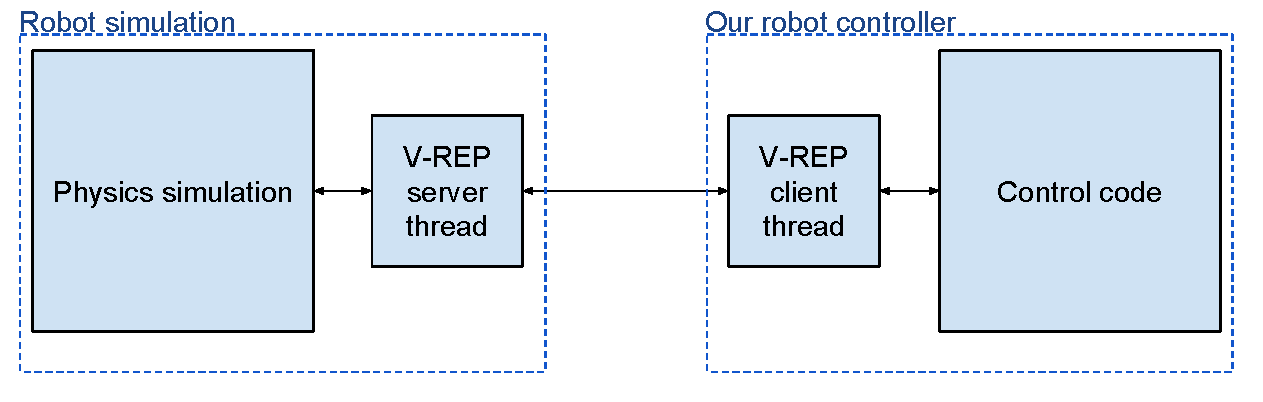
\includegraphics[width = \textwidth]{figures/simulation_principles}
    \caption[]{Representation of the architecture of the simulation setup. While the physics simulation is done in a simulator (V-Rep) along with the local control of the servos, the higher level control algorithms are executed outside. The communication between the simulator and high level control code is based on a TCP socket.}
    \label{fig:abstract1}
\end{figure}

\begin{figure}[htp]
\center
\begin{subfigure}[b]{0.45\textwidth}
    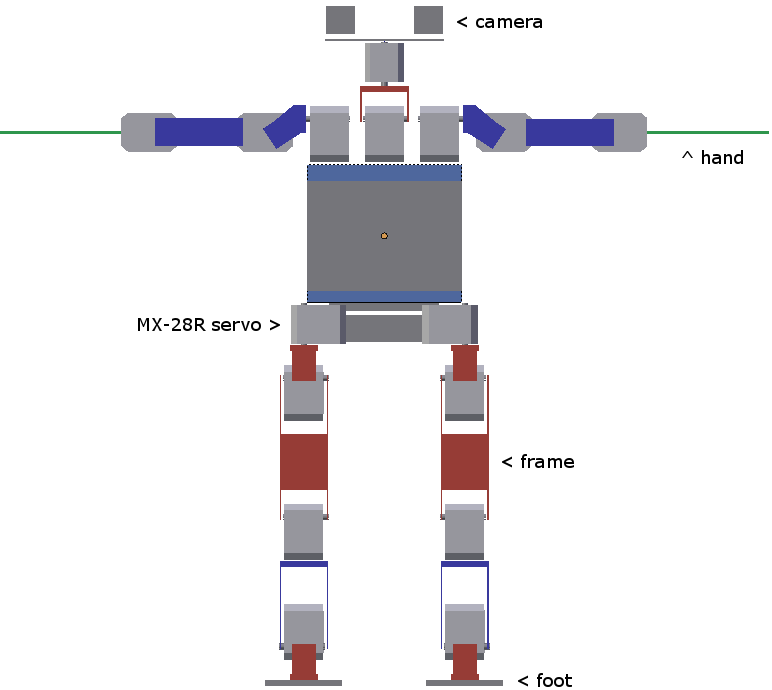
\includegraphics[width = \textwidth]{figures/robot_v7_front}
    \caption[]{Front view of the robot}
    \label{fig:abstract_robot1}
\end{subfigure}
\hfill
\begin{subfigure}[b]{0.45\textwidth}
\center
    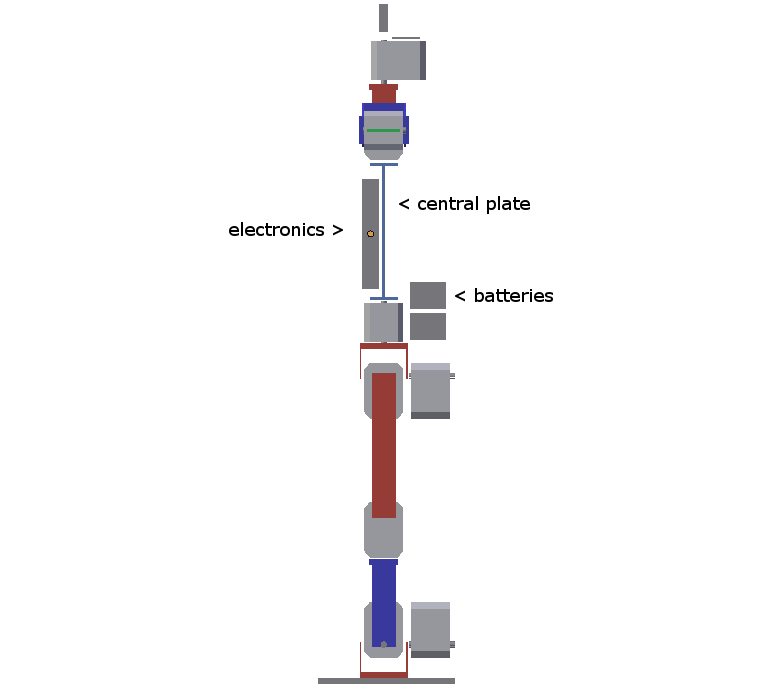
\includegraphics[width = \textwidth]{figures/robot_v7_side}
    \caption[]{Side view of the robot}
    \label{fig:abstract_robot2}
\end{subfigure}
\caption[]{Front and side views of the final robot design this master thesis produced. The servos (in grey) are connected together through different types of frames (in red and blue). At the top, two cameras are discernible and at the centre, the electronics and batteries can be seen.}
\label{fig:abstract2}
\end{figure}